\documentclass[11pt,a4paper]{article}
\usepackage[utf8]{inputenc}
\usepackage[T1]{fontenc}
\usepackage{amsfonts}
\usepackage{amssymb}
\usepackage{mdframed}
\usepackage{tikz}
\usepackage{tkz-tab}
\usepackage{pgfplots}
\usepackage{xcolor}
\usepackage{fancyhdr}
\usepackage{lastpage}
\usepackage[fleqn]{amsmath}
\setlength{\mathindent}{0pt}

% Défini les couleurs pour les graphiques
\definecolor{dark_green}{HTML}{008000}

% Extensions
\RequirePackage{geometry} 
\geometry{tmargin=1cm,bmargin=1.9cm,lmargin=1.9cm,rmargin=1.9cm}

% Paramètres du titre
\def\classe{$1^{\text{re}}$ Spécialité mathématiques}
\def\titre{Le second degré}
\def\theme{Algèbre - Cours}

% Paramètres de numérotation des pages
\fancypagestyle{custom}{
  \fancyhf{}
  \renewcommand{\headrulewidth}{0pt}
  \lfoot{Algèbre - Cours}
  \cfoot{Le second degré}
  \rfoot{\thepage/\pageref{LastPage}}
}

\usepackage{titlesec} % Pour personnaliser les titres
\usepackage{xcolor} % Pour définir des couleurs

\title{\titre}
\author{\classe \\ \theme}
\date{}

\renewcommand{\familydefault}{\sfdefault}

% Styles pour les mdframed
\mdfdefinestyle{definitionStyle}{
    leftline=true,
    rightline=false,
    topline=false,
    bottomline=false,
    linewidth=2pt,
    linecolor=black,
    innertopmargin=0pt,
    innerbottommargin=0pt,
    innerrightmargin=0pt,
    innerleftmargin=5pt,
}

\mdfdefinestyle{proprieteStyle}{
    linewidth=1pt,
    linecolor=black,
    innertopmargin=5pt,
    innerbottommargin=5pt,
    innerrightmargin=5pt,
    innerleftmargin=5pt,
}

% Supprime l'indentation des paragraphes
\setlength{\parindent}{0pt}

\begin{document}

\maketitle
\pagestyle{custom}
\thispagestyle{custom}

\section*{I. Les fonctions polynômes du second degré}

% Définition
\begin{mdframed}[style=definitionStyle]
	\textbf{Définition :} ~\\
	On appelle \emph{fonction polynôme (ou trinôme) du second degré} toute fonction $f$ définie sur $\mathbb{R}$ par ~\\
	$f(x)=ax^2+bx+c$ où $a$, $b$ et $c$ sont trois réel avec $a\not=0$. \\
	Les réels $a$, $b$ et $c$ sont appelés \emph{coefficients de la fonction.}
\end{mdframed}

\textbf{Exemple :}
\begin{itemize}
	\item $f$ définie sur $\mathbb{R}$ tel que $f(x)=2x^2-4x+1$
	\item $g$ définie sur $\mathbb{R}$ tel que $g(x)=-x^2+9x-12$
\end{itemize}

\textbf{Remarque :} L'expression $ax^2+bx+c$ est dite forme développée de $f(x)$.

\subsection*{1. Forme canonique}

% Théorème
\begin{mdframed}[style=proprieteStyle]
	\textbf{Théorème :} ~\\
	Toute fonction trinôme du second degré définie par $f(x)=ax^2+bx+c$ peut s'écrire sous une forme appelée
	canonique $f(x)=a(x-\alpha)^2+\beta$, avec $\alpha=-\frac{b}{2a}$ et $\beta=f(\alpha)$.
\end{mdframed}

\textbf{Exemple :} \\

Soit $f$ définie sur $\mathbb{R}$ par $f(x)=x^2-4x+17$. \\
Donner sa forme canonique.

\begin{enumerate}
	\item En utilisant le théorème :
	      On a $a=1$, $b=-4$ et $c=17$

	      Calculons $\alpha=-\frac{b}{2a}=-\frac{-4}{2\times1}=\frac{4}{2}=1$ et $\beta=f(\alpha)=f(2)=2^2-4\times2+17=13$

	      Donc la forme canonique de $f$ est $f(x)=1(x-2)^2+13$ pour tout $x\in\mathbb{R}$.

	\item En utilisant une identité remarquable :
	      \begin{flalign*}
		      f(x) & = x^2-4x+17     & \\
		           & = x^2-4x+4-4+17 & \\
		           & = (x-2)^2+13    &
	      \end{flalign*}

	      Donc la forme canonique de $f$ est $f(x)=(x-2)^2+13$ pour tout $x\in\mathbb{R}$.
\end{enumerate}

\newpage

\subsection*{2. Sens de variation}

\begin{mdframed}[style=proprieteStyle]
	\textbf{Propriété :} ~\\
	Soit $f$ une fonction définie sur $\mathbb{R}$ par $f(x)=a(x-\alpha)^2+\beta$.
	\begin{itemize}
		\item Cas où $a>0$ : la fonction $f$ est strictement décroissante sur $]-\infty;\alpha]$ puis strictement croissante sur $[\alpha;+\infty[$. $f$ admet un minimum égal à $\beta$ atteint en $x=\alpha$.
		\item Cas où $a<0$ : la fonction $f$ est strictement croissante sur $]-\infty;\alpha]$ puis strictement décroissante sur $[\alpha;+\infty[$. $f$ admet un maximum égal à $\beta$ atteint en $x=\alpha$.
	\end{itemize}
\end{mdframed}

\textbf{On retient :} ~\\
\begin{tabular}{@{}c@{\hspace{1cm}}c@{}}
	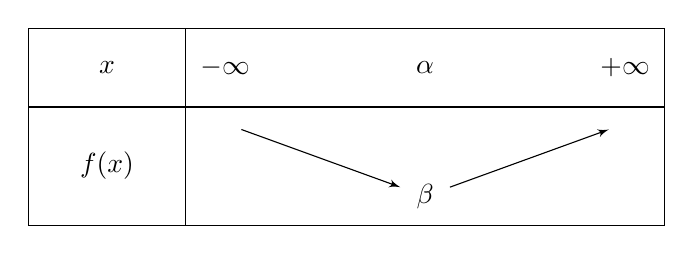
\begin{tikzpicture}[baseline, scale=1, transform shape]
		\tkzTabInit[lgt=2,espcl=2.54]{$x$ / 1 , $f(x)$ / 1.5}{$-\infty$, $\alpha$, $+\infty$}
		\tkzTabVar{+/ , -/ $\beta$, +/ }
	\end{tikzpicture} &
	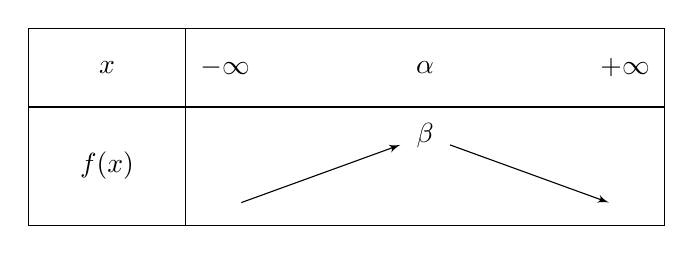
\begin{tikzpicture}[baseline, scale=1, transform shape]
		\tkzTabInit[lgt=2,espcl=2.54]{$x$ / 1 , $f(x)$ / 1.5}{$-\infty$, $\alpha$, $+\infty$}
		\tkzTabVar{-/ , +/ $\beta$, -/ }
	\end{tikzpicture}    \\
	\hspace{6.5cm} car $a > 0$                                                            &
	\hspace{6.5cm} car $a < 0$
\end{tabular}

\subsection*{3. Représentation graphique}

\begin{mdframed}[style=proprieteStyle]
	\textbf{Propriété \emph{(conséquence)} :} ~\\
	Soit $f$ une  fonction définie par $f(x)=a(x-\alpha)+\beta$. \\
	Dans un repère orthogonal d'origine $O$, la représentation graphique de la fonction $f$ est une parabole de sommet
	$S(\alpha;\beta)$ qui admet pour axe de symétrie la droite d'équation $x=\alpha$.
\end{mdframed}

\textbf{On retient :} ~\\

\begin{tabular}{@{}c@{\hspace{1cm}}c@{}}
	\begin{tikzpicture}
		\begin{axis}[
				axis lines=middle,
				xlabel={$x$},
				ylabel={$y$},
				xmin=-2, xmax=4,
				ymin=-2, ymax=4,
				xtick=\empty,
				ytick=\empty
			]
			\draw[dashed, thin, dark_green] (axis cs:1.833,-2) -- (axis cs:1.833,4);
			\draw[dashed, thin, blue] (axis cs:-2,-1.083) -- (axis cs:4,-1.083);
			\addplot[smooth, thick, red, domain=-2:4] {3*x^2 - 11*x + 9};
			\addplot[mark=x, mark size=3, only marks] coordinates {(1.833,-1.083)};
			\node[label={-30:$(\color{dark_green}\alpha\color{black},\color{blue}\beta\color{black})$}] at (axis cs:1.833,-1.083) {};
		\end{axis}
	\end{tikzpicture} &
	\begin{tikzpicture}
		\begin{axis}[
				axis lines=middle,
				xlabel={$x$},
				ylabel={$y$},
				xmin=-2, xmax=4,
				ymin=-2, ymax=4,
				xtick=\empty,
				ytick=\empty
			]
			\draw[dashed, thin, dark_green] (axis cs:1.25,-2) -- (axis cs:1.25,4);
			\draw[dashed, thin, blue] (axis cs:-2,3.125) -- (axis cs:4,3.125);
			\addplot[smooth, thick, red, domain=-2:4] {-2*x^2 + 5*x + 0};
			\addplot[mark=x, mark size=3, only marks] coordinates {(1.25,3.125)};
			\node[label={30:$(\color{dark_green}\alpha\color{black},\color{blue}\beta\color{black})$}] at (axis cs:1.25,3.125) {};
		\end{axis}
	\end{tikzpicture}   \\
	car $a > 0$               &
	car $a < 0$
\end{tabular}

\newpage

\section*{II. Factorisation d'une fonction du second degré et équation du second degré}

\subsection*{1. Factorisation}

\begin{mdframed}[style=definitionStyle]
	\textbf{Définition :} ~\\
	On appelle discriminant de la fonction trinôme $f:x \mapsto ax^2+bx+c$ ou de l'équation $ax^2+bx+c=0$ le réel $\Delta$ défini
	par $\Delta=b^2-4ac$.
\end{mdframed}


\textbf{Exemple :} Calculer le discriminant de l'équation $-3x^2+6x-3=0$. \\

On a $a=-3$, $b=6$ et $c=3$.
\begin{alignat*}{2}
	 & \text{Calculons} \quad & \Delta & = b^2-4ac                 \\
	 &                        &        & = 6^2 - 4\times(-3)\times(-3) \\
	 &                        &        & = 0
\end{alignat*}

% Théorème
\begin{mdframed}[style=proprieteStyle]
	\textbf{Théorème :} ~\\
	Soit $f$ sur $\mathbb{R}$ par $f(x)=ax^2+bx+c$.
	\begin{itemize}
		\item Si $\Delta<0$, alors $f(x)=ax^2+bx+c$ n'est pas factorisable.
		\item Si $\Delta=0$, alors $f(x)=a(x-\alpha)^2$ où $\alpha=-\frac{b}{2a}$.
		\item Si $\Delta>0$, alors $f(x)=a(x-x_1)(x-x_2)$ où $x_1=\frac{-b-\sqrt{\Delta}}{2a}$ et $x_2=\frac{-b+\sqrt{\Delta}}{2a}$.
	\end{itemize}
\end{mdframed}

\subsection*{2. Résolution des équation du second degré}

\begin{mdframed}[style=proprieteStyle]
	\textbf{Théorème :} ~\\
	Soit l'équation $ax^2+bx+c=0$ avec $a\not=0$:.
	\begin{itemize}
		\item Si $\Delta<0$, l'équation $ax^2+bx+c=0$ n'admet aucune solution.
		\item Si $\Delta=0$, l'équation $ax^2+bx+c=0$ admet une unique solution $\alpha=\frac{-b}{2a}$.
		\item Si $\Delta>0$, l'équation $ax^2+bx+c=0$ admet deux solutions distinctes : $x_1=\frac{-b-\sqrt{\Delta}}{2a}$ et $x_2=\frac{-b+\sqrt{\Delta}}{2a}$.
	\end{itemize}
\end{mdframed}

\textbf{Exemple :} Résoudre l'équation suivante $2x^2+19x+42=0$. \\

On a $a=2$, $b=19$ et $c=42$. \\
On calcule $\Delta=b^2-4ac=25$. \\
$\Delta>0$ donc l'équation admet deux solutions. \\
$x_1=\frac{-b-\sqrt{\Delta}}{2a}=\frac{-19-\sqrt{25}}{2\times2}=-6$ \\
$x_2=\frac{-b+\sqrt{\Delta}}{2a}=\frac{-19+\sqrt{25}}{2\times2}=-\frac{7}{2}$ \\
L'ensemble solution est $S=\{-6;-\frac{7}{2}\}$. \\

\subsection*{3. Somme et produit des racines}

\begin{mdframed}[style=proprieteStyle]
	\textbf{Propriété :} ~\\
	Soit $x_1$ et $x_2$ les racines d'une fonction polynôme du second degré $ax^2+bx+c$, avec $a\not=0$. \\
	On a alors $x_1+x_2=-\frac{b}{a}$ et $x_1\times x_2=\frac{c}{a}$
\end{mdframed}

\newpage

\section*{III. Signe d'une fonction du second degré et inéquations}

\begin{tabular}{@{}c@{\hspace{1cm}}c@{}}
	\fbox{\begin{minipage}{0.45\textwidth}
			      \centering
			      $a > 0$ et $\Delta<0$\\
			      \resizebox{0.5\textwidth}{!}{
				      \begin{tikzpicture}
					\begin{axis}[
							axis lines=middle,
							hide y axis,
							xlabel=$x$,
							xlabel style={font=\huge},
							samples=101,
							domain=-4:4,
							xmin=-4, xmax=4,
							ymin=-1, ymax=15,
							xtick=\empty,
							ytick=\empty
						]
						\addplot[red, very thick] {x^2+2};
					\end{axis}
				\end{tikzpicture}} \\
			      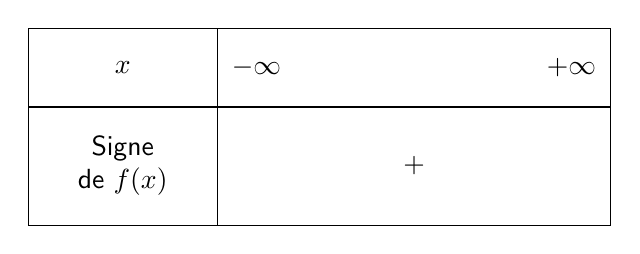
\begin{tikzpicture}[baseline, scale=1, transform shape]
				\tkzTabInit[lgt=2.4,espcl=4]{$x$ / 1 , Signe de $f(x)$ / 1.5}{$-\infty$, $+\infty$}
				\tkzTabLine{, +, }
			\end{tikzpicture}
		      \end{minipage}} &
	\fbox{\begin{minipage}{0.45\textwidth}
			      \centering
			      $a < 0$ et $\Delta<0$\\
			      \resizebox{0.5\textwidth}{!}{
				      \begin{tikzpicture}
					\begin{axis}[
							axis lines=middle,
							hide y axis,
							xlabel=$x$,
							xlabel style={font=\huge},
							samples=101,
							domain=-4:4,
							xmin=-4, xmax=4,
							ymin=-15, ymax=1,
							xtick=\empty,
							ytick=\empty
						]
						\addplot[red, very thick] {-x^2-2};
					\end{axis}
				\end{tikzpicture}} \\
			      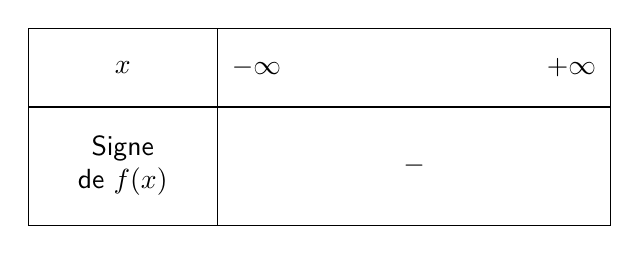
\begin{tikzpicture}[baseline, scale=1, transform shape]
				\tkzTabInit[lgt=2.4,espcl=4]{$x$ / 1 , Signe de $f(x)$ / 1.5}{$-\infty$, $+\infty$}
				\tkzTabLine{, -, }
			\end{tikzpicture}
		      \end{minipage}} \\
	\fbox{\begin{minipage}{0.45\textwidth}
			      \center
			      $a > 0$ et $\Delta=0$\\
			      \resizebox{0.5\textwidth}{!}{
				      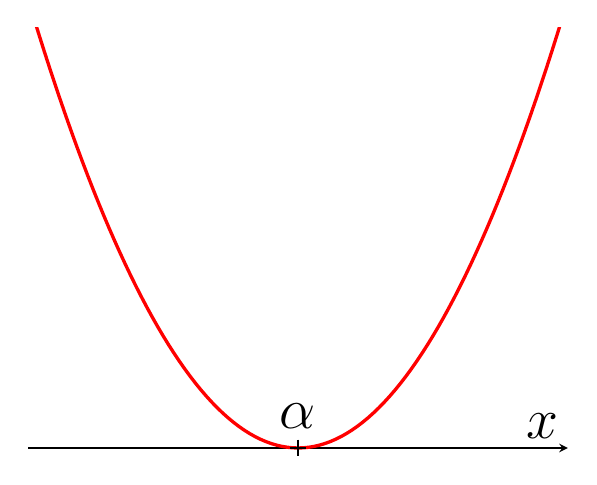
\begin{tikzpicture}
					\begin{axis}[
							axis lines=middle,
							hide y axis,
							xlabel=$x$,
							xlabel style={font=\huge},
							samples=101,
							domain=-4:4,
							xmin=-4, xmax=4,
							ymin=-1, ymax=15,
							xtick=\empty,
							ytick=\empty,
						]
						\addplot[red, very thick] {x^2};
						\addplot[mark=+, mark size=3, only marks] coordinates {(0,0)};
						\node[label={[font=\huge]90:$\alpha$}] at (axis cs:0,0) {};
					\end{axis}
				\end{tikzpicture}} \\
			      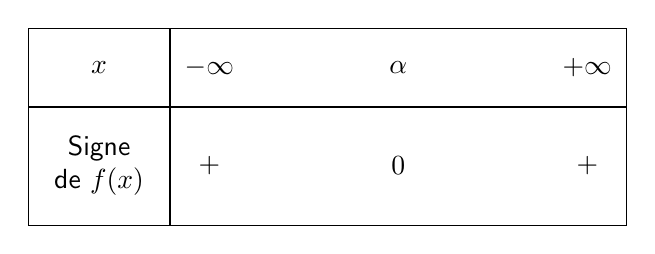
\begin{tikzpicture}[baseline, scale=1, transform shape]
				\tkzTabInit[lgt=1.8,espcl=2.4]{$x$ / 1 , Signe de $f(x)$ / 1.5}{$-\infty$, $\alpha$, $+\infty$}
				\tkzTabLine{+, , 0, , +}
			\end{tikzpicture}
		      \end{minipage}} &
	\fbox{\begin{minipage}{0.45\textwidth}
			      \center
			      $a < 0$ et $\Delta=0$\\
			      \resizebox{0.5\textwidth}{!}{
				      \begin{tikzpicture}
					\begin{axis}[
							axis lines=middle,
							hide y axis,
							xlabel=$x$,
							xlabel style={font=\huge},
							samples=101,
							domain=-4:4,
							xmin=-4, xmax=4,
							ymin=-15, ymax=1,
							xtick=\empty,
							ytick=\empty
						]
						\addplot[red, very thick] {-x^2};
						\addplot[mark=+, mark size=3, only marks] coordinates {(0,0)};
						\node[label={[font=\huge]-90:$\alpha$}] at (axis cs:0,0) {};
					\end{axis}
				\end{tikzpicture}} \\
			      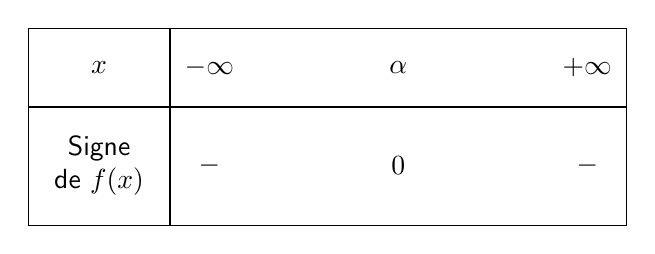
\begin{tikzpicture}[baseline, scale=1, transform shape]
				\tkzTabInit[lgt=1.8,espcl=2.4]{$x$ / 1 , Signe de $f(x)$ / 1.5}{$-\infty$, $\alpha$, $+\infty$}
				\tkzTabLine{-, , 0, , -}
			\end{tikzpicture}
		      \end{minipage}} \\
	\fbox{\begin{minipage}{0.45\textwidth}
			      \center
			      $a > 0$ et $\Delta>0$\\
			      \resizebox{0.5\textwidth}{!}{
				      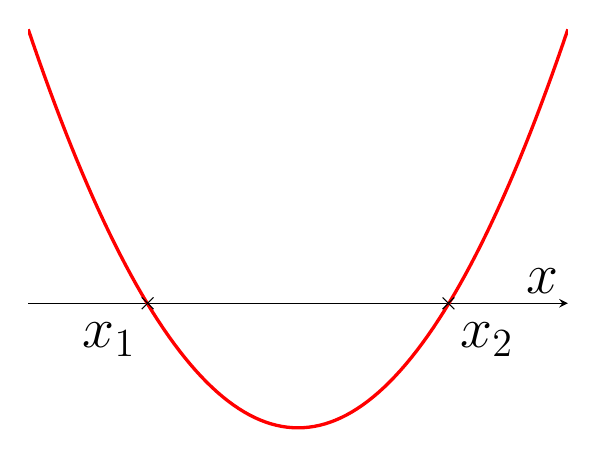
\begin{tikzpicture}
					\begin{axis}[
							axis lines=middle,
							hide y axis,
							xlabel=$x$,
							xlabel style={font=\huge},
							samples=101,
							domain=-4:4,
							xmin=-4, xmax=4,
							ymin=-6, ymax=12,
							xtick=\empty,
							ytick=\empty
						]
						\addplot[red, very thick] {x^2-5};
						\addplot[mark=x, mark size=3, only marks] coordinates {(2.23,0)};
						\node[label={[font=\huge]-90:$x_2$}] at (axis cs:2.8,0) {};
						\addplot[mark=x, mark size=3, only marks] coordinates {(-2.23,0)};
						\node[label={[font=\huge]-90:$x_1$}] at (axis cs:-2.8,0) {};
					\end{axis}
				\end{tikzpicture}}\\
			      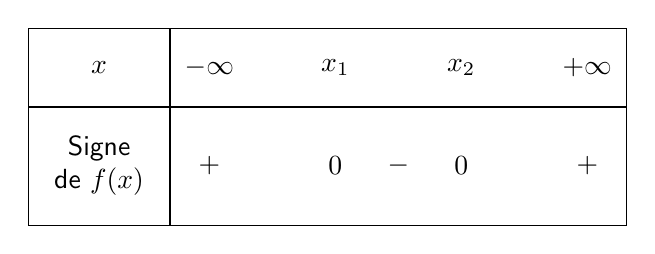
\begin{tikzpicture}[baseline, scale=1, transform shape]
				\tkzTabInit[lgt=1.8,espcl=1.6]{$x$ / 1 , Signe de $f(x)$ / 1.5}{$-\infty$, $x_1$, $x_2$, $+\infty$}
				\tkzTabLine{+, , 0, -, 0, , +}
			\end{tikzpicture}
		      \end{minipage}} &
	\fbox{\begin{minipage}{0.45\textwidth}
			      \center
			      $a < 0$ et $\Delta>0$\\
			      \resizebox{0.5\textwidth}{!}{
				      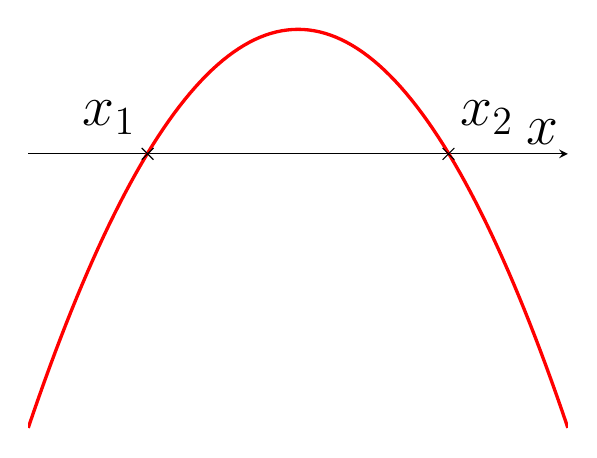
\begin{tikzpicture}
					\begin{axis}[
							axis lines=middle,
							hide y axis,
							xlabel=$x$,
							xlabel style={font=\huge},
							samples=101,
							domain=-4:4,
							xmin=-4, xmax=4,
							ymin=-12, ymax=6,
							xtick=\empty,
							ytick=\empty
						]
						\addplot[red, very thick] {-x^2+5};
						\addplot[mark=x, mark size=3, only marks] coordinates {(2.23,0)};
						\node[label={[font=\huge]90:$x_2$}] at (axis cs:2.8,0) {};
						\addplot[mark=x, mark size=3, only marks] coordinates {(-2.23,0)};
						\node[label={[font=\huge]90:$x_1$}] at (axis cs:-2.8,0) {};
					\end{axis}
				\end{tikzpicture}} \\
			      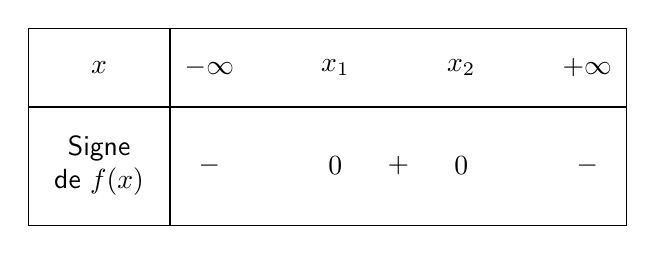
\begin{tikzpicture}[baseline, scale=1, transform shape]
				\tkzTabInit[lgt=1.8,espcl=1.6]{$x$ / 1 , Signe de $f(x)$ / 1.5}{$-\infty$, $x_1$, $x_2$, $+\infty$}
				\tkzTabLine{-, , 0, +, 0, , -}
			\end{tikzpicture}
		      \end{minipage}}
\end{tabular}

\begin{mdframed}[style=proprieteStyle]
	\textbf{Propriété :} ~\\
	Soit $f$ définie sur $\mathbb{R}$ par $f(x)=ax^2+bx+c$.
	\begin{itemize}
		\item Si $\Delta<0$, alors pour tout réel $x$, $f(x)$ est du signe de $a$.
		\item Si $\Delta=0$, alors pour tout réel $x$, $f(x)$ est du signe de $a$ sauf en $\alpha$ où $x$ vaut $0$.
		\item Si $\Delta>0$, alors pour tout réel $x$, $f(x)$ s'annule en $x_1$ et $x_2$ et est du signe de $a$ pour 
		tout $x\in]-\infty;x_1[\cup]x_2;+\infty[$ (avec $x_1<x_2$) et du signe opposé à celui de $a$ pour tout $x\in]x_1;x_2[$.
	\end{itemize}
\end{mdframed}
\textbf{Remarque :} On peut retenir que $f(x)$ est du signe de $a$ sauf entre les racines lorsqu'elles existent.



\end{document}